% !TEX encoding = UTF-8
% !TEX program = pdflatex
% !TEX spellcheck = en_GB

\documentclass[english,a4paper]{europasscv}
\usepackage[english]{babel}
\usepackage{pdfpages}

\ecvname{Salvador Martin}
\ecvaddress{Via Antrodoco 1, 67100, AQ (Italy)}
\ecvmobile{+39 380 193 1121}
%\ecvtelephone{+353 127 6689}
%\ecvworkphone{+353 999 888 777}
\ecvemail{salvador.martin.cu@gmail.com}
%\ecvhomepage{www.myhomepage.com www.another-homepage.com}
% \ecvgithubpage{www.github.com/smith}
\ecvlinkedinpage{www.linkedin.com/in/salvador-martin}
%\ecvim{AOL Messenger}{katie.smith}
%\ecvim{Google Talk}{ksmith}
\ecvim{Skype}{salva2015cu}

\ecvdateofbirth{20 January 1983}
\ecvnationality{Cuban}
\ecvgender{Male}

\ecvpicture[width=2.8cm]{yo}

\date{}

\begin{document}
  \begin{europasscv}

  \ecvpersonalinfo

%\ecvbigitem{Job applied for}{Product Engineer}

  \ecvsection{Work experience}
  \ecvtitle{Dec, 2013 -- Sep, 2015}{Computer Network Administrator}
  \ecvitem{}{University of Matanzas ''Camilo Cienfuegos'', Matanzas (Cuba)}
  \ecvitem{}{
 	\begin{ecvitemize}
 		\item Development, design, optimization and maintenance of the university computer network,
 		\item Configuration and maintenance of switchers, routers and communication equipment,
 		\item Optimization and maintenance of the computer network services (DNS, DHCP, Web Servers (IIS, Apache), Network Proxy (IPTables, ISA Server, Squeeze), Active Directory (Linux and Windows), e--mail Service),
 		\item Installation, configuration and maintenance of dedicated servers over Windows or Linux Distribution (Phisycally located$/$Cloud located),
 		\item Instalation, configuration and maintenance of workstations dedicated to the services of the university.
 	\end{ecvitemize}
  }
  \ecvtitle{Sep, 2011 -- Sep, 2015}{Professor}
  \ecvitem{}{University of Matanzas ''Camilo Cienfuegos'', Matanzas (Cuba)}
  \ecvitem{Assistant Professor,\qquad \qquad \qquad \qquad Sep, 2013 -- Sep, 2015}{
 	\begin{ecvitemize}
 		\item Carrying out the preparation and teaching jointly with the main professor of the subject Thermodynamic Technologies 1 and 2, to the third year of the Mechanical Engineering Degree,
 		\item Professor of the subject of Principles of Renewable Energies in the Mechanical Engineering Degree,
 		\item Collaboration in the Construction Engineering Degree, teaching the Basis of Renewable Energies,
 		\item Collaboration in the Industrial Engineering Degree, teaching the subject Technological Processes.
  	\end{ecvitemize}
  } 
  \ecvitem{Professor in Instruction, \qquad \qquad Sep, 2012 -- Sep, 2013}{
 	Began and success preparation as university professor performing jointly with my supervisor, the preparation and realization of the subjects Thermodynamic Technologies 1 and 2, to the third year of the Mechanical Engineering.
 	}
  \ecvitem{Associate Professor \qquad \qquad \qquad \qquad  Sep, 2011 -- Sep, 2012}{
  	Teaching the lectures of the subject Information Systems in the Accounting and Finances Degree. The main objective of this lecture is to equip future accountants with basic knowledge on the proper codification and computer encryption of accounting information, as well as tools and techniques for its implementation.	
 	}  
  \ecvitem{General activities}{
  	\begin{ecvitemize}
  		\item To mentor$/$follow students research on different relevant fields linked to the line of research of the faculty Mechanical Engineer,
  		\item To prepare, design and present research projects to the scientific council of the faculty of Mechanical Engineering,
  		\item To organize and execute the field work with the students, in the industries in the territory, with the main objective of relating them to the reality of the technological facilities and the execution and solution of assigned tasks,
  		\item To participate in thesis defense sessions as an opponent of thesis, jury or thesis supervisor. 
  	\end{ecvitemize}
  }
  \ecvtitle{Mar 2007 -- Sep 2011}{Computer, Network \& IT security consultant}
  \ecvitem{}{Specialized Protection Services S.A (SEPSA), Matanzas (Cuba)}
  \ecvitem{}{Carrying out detailed study and evaluation of information flow, trace analysis and detection of faults and vulnerabilities on the computer network. Realization of diagnostics (GFI Languard, Tenable Nessus), as well as the redesign of the computer system network with the implementation of intruders detection systems (IDS) and protection against cyber--attacks from$/$and to the local computer network to third companies.}
    
  \ecvsection{Education and training}
  \ecvtitlelevel{Sep 2015 -- Now}{PhD (ongoing)}{}
  \ecvitem{\textbf{Thesis Title}}{Smart grids: Fault and attack detection, and robust control design.}
  \ecvitem{\textbf{Director}}{Stefano Di Gennaro}
  \ecvitem{}{Università degli Studi dell'Aquila, L'Aquila (Italy)}
  \ecvtitlelevel{2004 -- 2009}{Mechanical Engineering Degree}{}
  \ecvitem{\textbf{Thesis title}}{Proposal of a photovoltaic system for the supply of electricity to the main consumers of the rectory of the University of Matanzas ''Camilo Cienfuegos''}
  \ecvitem{\textbf{Director}}{Ju\'an I. V\'eliz Alonso}
  \ecvitem{}{University of Matanzas, Matanzas (Cuba)}
  
  \ecvsection{Personal skills}
  \ecvmothertongue{Spanish}
  \ecvlanguageheader
  \ecvlanguage{English}{B1}{B2}{B2}{B1}{B1}
  \ecvlastlanguage{Italian}{B2}{B2}{B2}{B1}{B1}
  \ecvlanguagefooter
   
  \ecvblueitem{Communication skills}{
  \begin{ecvitemize}
  	\item I am a volunteer of Erasmus Students Network (ESN)--Aquilasmus helping new Erasmus students, promoting and organizing as part of the team, differents extracurricular activities
  	\item During my Ph.D. research I have been working and collaborating with others Ph.D. students from different fields. 
  \end{ecvitemize}
  }
  \ecvblueitem{Organisational$/$managerial skills}{
  \begin{ecvitemize}
    \item Whilst working as a professor on University of Matanzas ''Camilo Cienfuegos'', I was in charge of the management and organization of activities with students, inside and outside the classroom,
    \item Management and organization of research projects and student's thesis management,
    \item Whilst working as Computers Network Security Consultant, I was in charge of making presentations with the executives of the companies that hired my services, where advice was given on good practices in the use of ICT, in addition to of the commercial management and promotion of the service.
  \end{ecvitemize}
  }

  %\ecvdigitalcompetence{\ecvBasic}{\ecvIndependent}{\ecvProficient}{\ecvIndependent}{\ecvBasic}
  
  \ecvblueitem{Computer skills}{\textbf{General purpose}}{}
  \ecvitem{}{Microsoft Office, Open Office, Libre Office}{}
  \ecvitem{}{\textbf{Operative Systems}}{}
  \ecvitem{}{Microsoft Windows, Linux (Debian, Ubuntu, SUSE)}{}
  \ecvitem{}{\textbf{Design and sketching}}{}
  \ecvitem{}{AutoCAD, Mechanical Desktop, Adobe Fireworks, TKSolver}{}
  \ecvitem{}{\textbf{Programming and simulation}}{}
  \ecvitem{}{Matlab, Simulink, Latex, TKSolver, HTML, PHP}{}
  \ecvitem{}{\textbf{Computers Network Management}}{}
  \ecvitem{}{DNS, DHCP, Web Servers (IIS, Apache), Network Proxy (IPTables, ISA Server, Squeeze), Active Directory (Linux and Windows), e--mail Service, Virtual Machines (VM Ware, VirtualBox)}{}
    
  \ecvblueitem{Other skills}{In my free time I like to read a book, to meet my friends and pass time with them dancing or cathing up, to listen good music: salsa, merengue, bachata, old classics, blues, R\&B, Jazz. My passions are to practice sports: to swim, to train martial Arts, to play any game in general.}

  \ecvblueitem{Driving licence}{A, B}
  
  \ecvsection{Additional information}
  \ecvbigitem{Advanced Courses}{}
  \ecvtitle{2017}{Formal Methods for the Control of Large-scale Networked Nonlinear Systems with Logic Specifications}
  \ecvitem{}{by Alessandro Borri, Maria Domenica Di Benedetto, Giordano Pola and Pierdomenico Pepe}
  \ecvitem{}{Università degli Studi dell'Aquila, L'Aquila (Italy)}
  \ecvtitle{}{7th oCPS PhD School on Cyber-Physical Systems}
  \ecvitem{}{IMT School for Advanced Studies, Lucca (Italy)}
  \ecvtitle{}{Energy-based modeling and control of physical system}
  \ecvitem{}{by Arjan van der Schaft (University of Groningen) and Dimitri Jeltsema (TU Delft (Netherland))}
  \ecvitem{}{CentraleSupélec, Paris (France)}
  \ecvtitle{2016}{Tools for nonlinear control, Lyapunov function, positivity, applications}
  \ecvitem{}{by Frédéric Mazenc (CentraleSupélec (France))}
  \ecvitem{}{Università degli Studi dell'Aquila, L'Aquila (Italy)}
  \ecvtitle{}{Cyber-Physical systems control: Algebraic and Optimization techniques}
  \ecvitem{}{by Raphaël Jungers (UCL (Belgium))}
  \ecvitem{}{Università degli Studi dell'Aquila, L'Aquila (Italy)}
    
  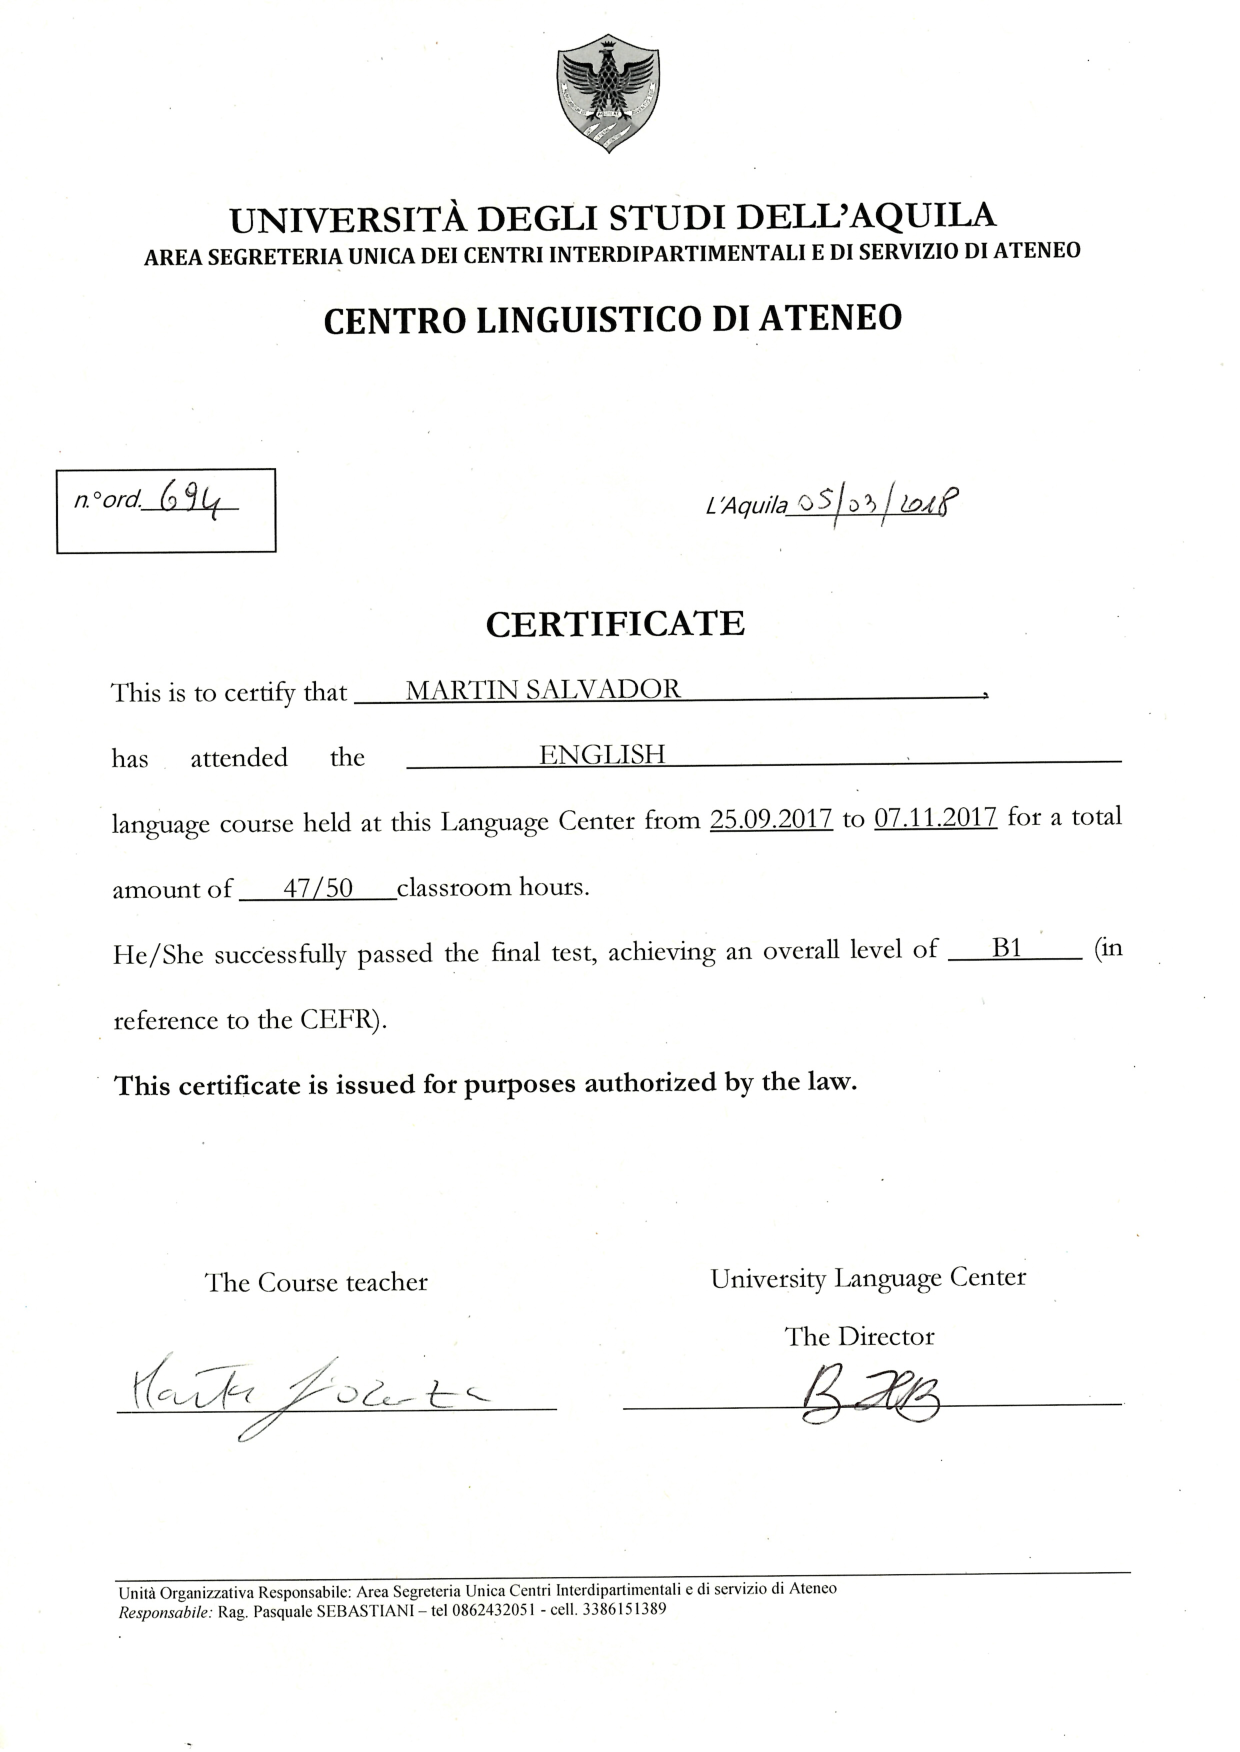
\includepdf{English(en)}
  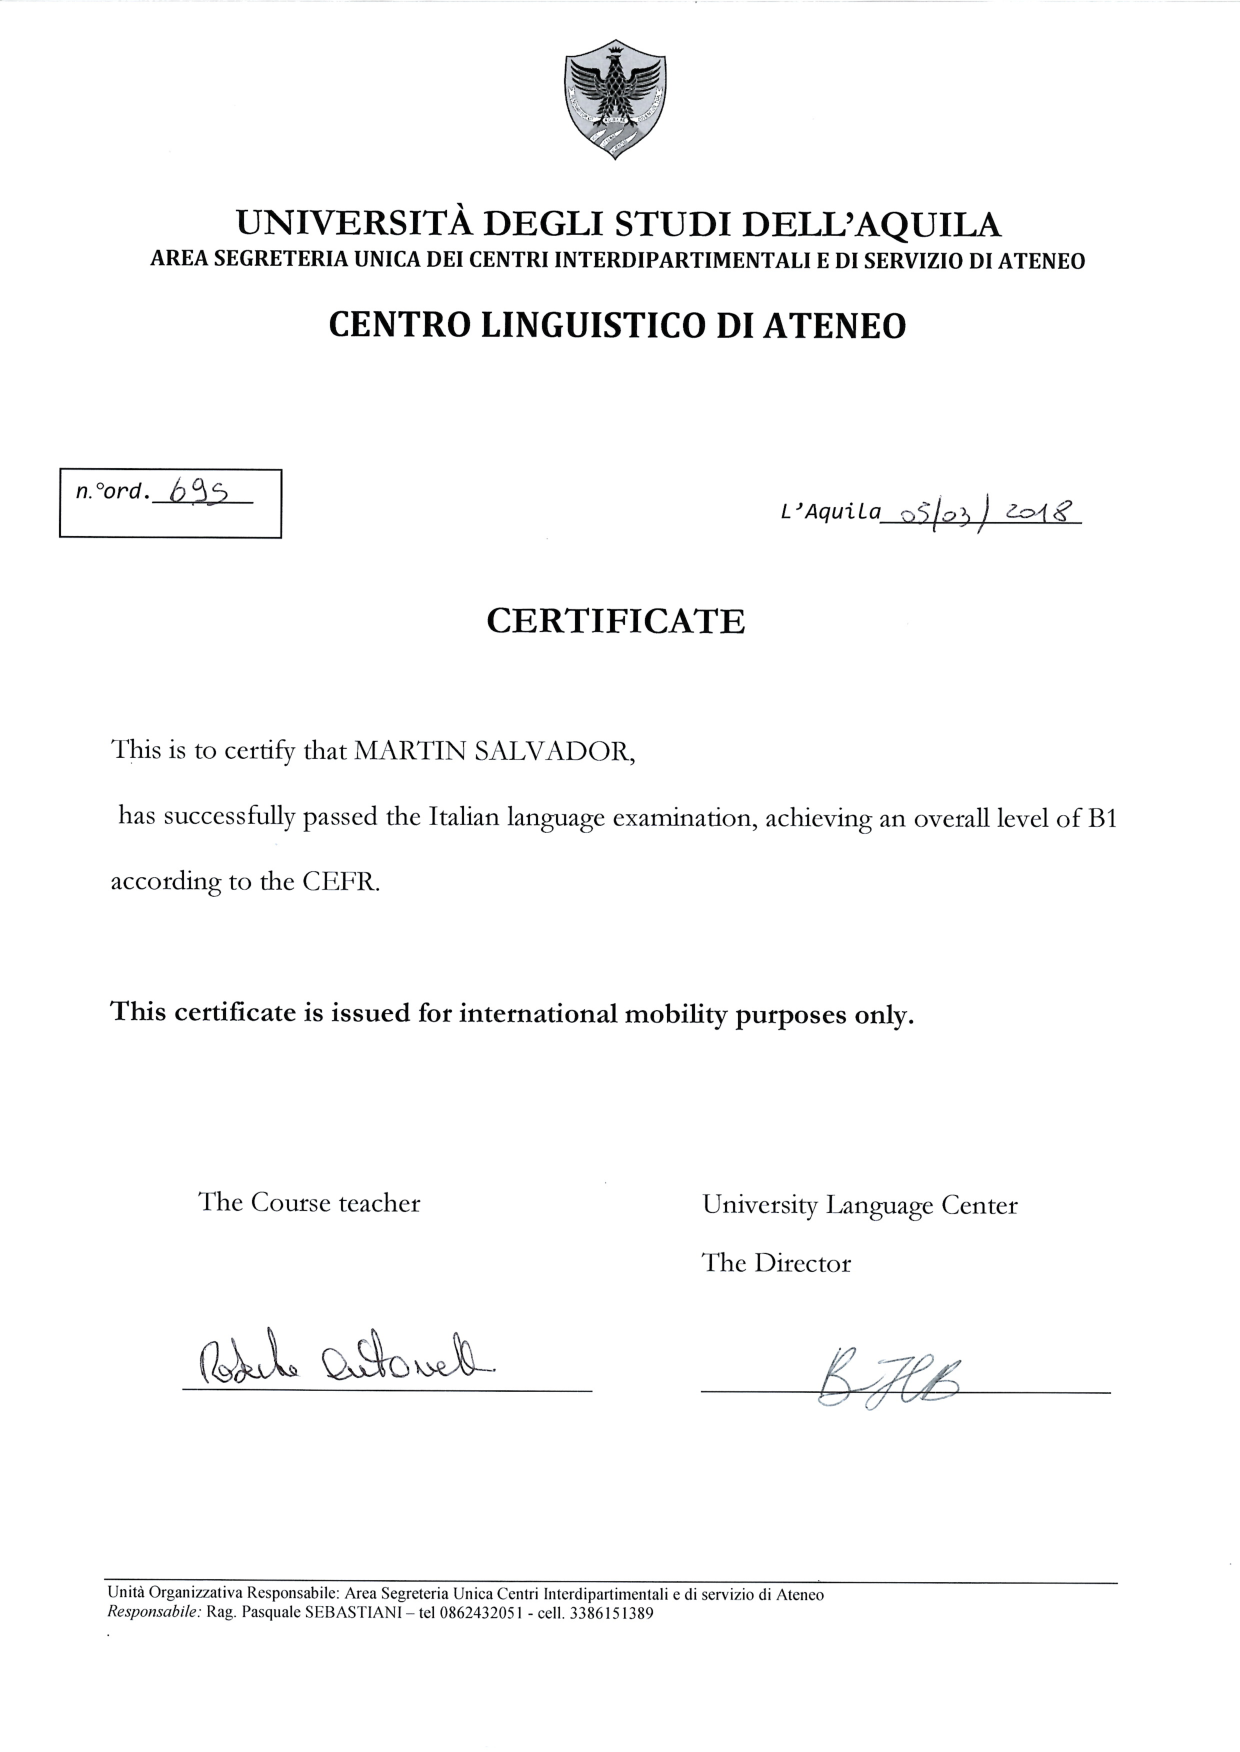
\includepdf{Italian(en)}
  \end{europasscv}

\end{document}